\begin{figure}[htp]
  \centering
  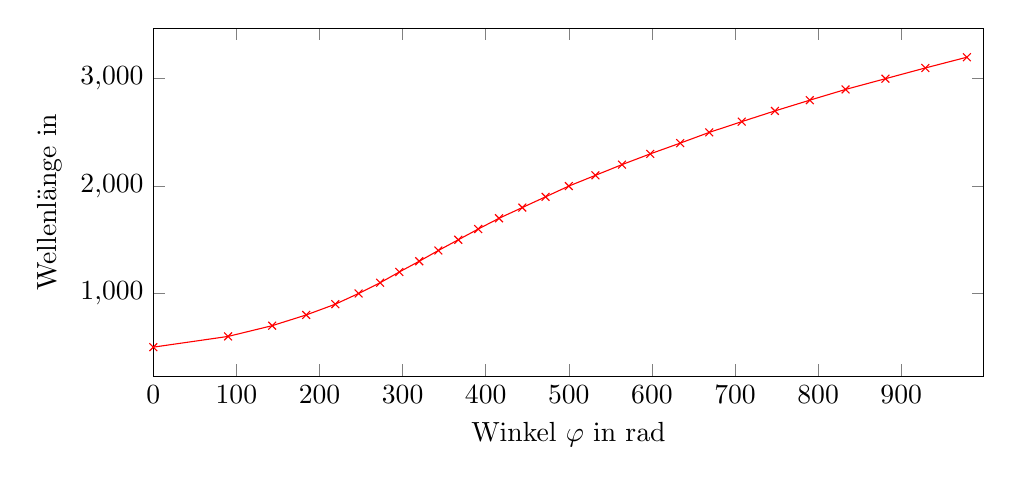
\begin{tikzpicture}
    \begin{axis}[disabledatascaling, width=\textwidth, height=6cm, ylabel=Wellenlänge in \si{\nano\metre}, xlabel=Winkel  $\varphi$ in rad, xmin = 0, xmax=999, xtick={}]
      \addplot[color=red,mark=x] coordinates {
		(0,500)
    (90,600)
		(143,700)
		(184,800)
    (219,900)
    (247,1000)
    (273,1100)
    (296,1200)
    (320,1300)
    (343,1400)
    (367,1500)
    (391,1600)
    (416,1700)
    (444,1800)
    (472,1900)
    (500,2000)
    (532,2100)
    (564,2200)
    (598,2300)
    (634,2400)
    (669,2500)
    (708,2600)
    (748,2700)
    (790,2800)
    (833,2900)
    (881,3000)
    (929,3100)
    (979,3200)
	};
    \end{axis}
  \end{tikzpicture}
\end{figure}
